\documentclass[11pt,UKenglish, a4paper]{article}
\usepackage[utf8]{inputenc}
%--fonts--
\usepackage[T1]{fontenc}
\usepackage[bitstream-charter]{mathdesign}

%--packages--
\usepackage[UKenglish]{babel}
\usepackage{csquotes,textcomp,varioref}

\usepackage{graphicx}
%--color--
\usepackage[dvipsnames]{xcolor}

%Setter inn pdfer
\usepackage[final]{pdfpages}

%-linespace--
\linespread{1.3}

%-Mer advansert liste--
\usepackage{enumitem}

%--hyperlinks-- include 
\usepackage[colorlinks=false, pdfborder={0 0 0}]{hyperref}

%--include subfiles-- 
\usepackage{subfiles}

%--fullpage--
%\usepackage{fullpage}

%--Uio-Front-Page--
%removed until it works \usepackage{ifikompendiumforside}

%--bibliography- -sortlocale=nb_No,
\usepackage[backend=biber, sortcites, defernumbers, style=numeric-comp, maxnames=2, natbib=true, backref, sorting=none, url=false]{biblatex}
%fjernet ifra style=authoryear-icomp
\addbibresource[datatype=bibtex]{Remote.bib}

%farger jeg skal ha med
\definecolor{myY}{RGB}{241, 196, 15}
\definecolor{myB}{RGB}{52, 152, 219}
\definecolor{myG}{RGB}{46, 204, 113}
\definecolor{myLy}{RGB}{149, 165, 166}
\definecolor{myR}{rgb}{231, 76, 60}

%--Author and Title--
\author{Simon Lysne Hyenes}
\title{Thematic Analysis}

%--Latex Optimalization--
\tolerance = 5000
\hbadness = \tolerance
\pretolerance = 2000

%--Starter--
\begin{document}

\section{Thematic Analysis}
In qualitative studies there are a range of options for analysis and gaining a deeper understanding of the data. Thematic analysis is described by Braun and Clarke as a method for ``identifying, analysOther possibilities were not expanded upon due to the lenght of the interview.ing, and reporting patterns (themes) within data''\cite[p.79]{Braun2006Using}. Thematic analysis is described as a theoretically flexible method, open for different theoretical approaches. This flexibility means that the researchers have to carefully describe their approach and the decisions made before, during and after the analysis. 

\subsection{Phases of thematic analysis}
Braune and Clarke's account gives a clear description of the method and divides it into 6 phases. In phase 1 the goal is to ``familiarize yourself with the data''\cite[p.87]{Braun2006Using}. This involves transcribing, reading and starting to form ideas about how to approach the data. 

\paragraph{}In phase 2 the researcher should have an inclination towards what is interesting and present in the dataset. This allows the researcher to code segments which are interesting or pertinent. The idea is to analyse the entire dataset in a similar manner---``giving full and equal attention to each data item''\cite[p.89]{Braun2006Using}. The actual coding process should be done systematically but the tools may range from pen and post-it notes to spreadsheets. Coding should be done liberally including as many themes and codes as feasible, include contextual information and allow for multiple codes on data item\cite[p.89]{Braun2006Using}.

\paragraph{}In phase 3 the codes should be systematically considered for broader themes. In so each code may be considered and combined with others to form higher themes in the dataset. Braun and Clarke recommend using visual techniques such as mindmaps, tables and card-sorting. The thematic map is then a mindmap including themes, subthemes and relations between the themes. Codes should be within the thematic groups but there may still be codes that aren't grouped.

\paragraph{}In phase 4 the themes are again considered, the ``candidate themes''\cite[p.91]{Braun2006Using} may be combined, split or otherwise rearranged. To do this systematically Braun and Clarke point to Patton's ``internal homogenity and external heterogenity''\cite[p.91]{Braun2006Using}. The themes should be internally logical and in comparison clearly separate. This is done by first considering the codes within each theme to analyse if they are consistent and form a meaningful theme. The second phase is ready when all the candidate themes are ready. The overall themes are then considered in relation to the entire dataset. Here the themes should be considered to what degree they capture and represent the whole. Each theme and the whole set of themes should be considered. The idea is to rework the themes until they can form a thematic map that gives an ``accurate representation''\cite[p.91]{Braun2006Using}. 

\paragraph{}Phase 5 involves naming and further defining themes. This involves a process in which the goal is to ``define and then further refine''\cite[p.92]{Braun2006Using} each theme. The idea is to gain a deeper understanding of what the theme's ``essence''\cite[p.92]{Braun2006Using} is. Here the themes may be considered for sub-themes. 

\paragraph{}Phase 6 is writing and producing a report, the report should be a consistent narrative of the data and analysis ``which convinces the reader of the merit and validity of your analysis''\cite[p.93]{Braun2006Using}. Here extracts and quotes that highlight interesting aspect should be used to ``go beyond description of the data, and make an argument in relation to your research question''\cite[p.93]{Braun2006Using}.

The phases are all closely related and describe an iterative process of working and reworking the dataset. The first 5 phases all involve moving forwards by reworking previous results. The phases are however useful to focus and promote analytical robustness. It also allows for a systematic way to describe why and how each phase was concluded. There is also a lack of clarity when it comes to finishing recoding codes and reworking themes. The only way to finish is by determining if there is little utility in continued analysis\cite[p.92]{Braun2006Using}.

\subsection{Workshop 1} 
For workshop 1 the dataset consisted of the interviews and the drawings. During the first thematic analysis the drawings were only used to consider the codes and inform what they participants were describing. In phase 1 the interviews were transcribed using standard procedures for anonymizing the data. In transcribing the interviews we are refamiliarized with the discussion and also gain insight into the general ideas and topics. It may be done as a purely mechanical exercise. Braun and Clarke however point to the ``interpretive''\cite[p.88]{Braun2006Using} qualitites of transcribing. The act of transcribing involves recording and bringing forwards non-verbal and contextual information. For instance persons entering or leaving the room, multiple conversations, irony, sarcasm, body-language. The goal is to have a rich dataset without the context being ``lost-in-translation''. In transcribing the interviews I attempted to include all such pertinent information. An example was in the drawing exercise pauses and quiet moments where also transcribed. Without it being clear that the participants are drawing the conversation during and after may be nonsensical. For phase 1 the transcription means establishing a bond with the dataset. Several ideas about the dataset became clear but also several problems became apparent. 

It became clear that the dataset was heavily reliant on the participatory sketching exercise which took a longer portion of time than planned. In the introduction and the beginning of the exercise the data is more pratical than descriptive. The interviews were with groups of respectively 2, 3 and 3 participants. Each group had 20 minutes, within this alloted time there was barely time to gage the participants. Much of the interviews are thin of rich descriptive statements. This would be worse if the interviews was the entire dataset, the sketches however give a deeper insight. 

\paragraph{}After the data was transcribed and reread several times I started phase 2. Here I focused on finding interesting excerpts of opinions, statements and other relevant data. This was coded liberally with several terms and phrases. For each group I first manually annotated and highlighted the interviews using a pen and a marker. With a second copy I did this again using the most useful codes from the first time but also including new codes. The codes were then included in a spreadsheet with the quotations and a remark about the data. 
From here I started phase 3 which involved sorting through all the codes and trying to find themes that would describe them. The themes should be seen in relation to the research question. The themes are not considered on prevalence alone but on their ability to describe important properties of the dataset in relation to the research questions\cite[]{Braun2006Using}. During this phase a major effort was to allow interal contradictions and include data items that didn't fit within the larger themes. 

\paragraph*{}In phase 4 and 5 the themes and their relation to the dataset was considered. It became clear that there was a large number of subthemes that could easily intersect or fit within multiple themes. Separating and sorting the themes was a bit troublesome since so many of the data items had been coded with more than one code. In phase 4 and 5 I worked the following thematic map showing the themes and subthemes as three separate blocks. 
\begin{figure}[Thematic Map]
    \centering
	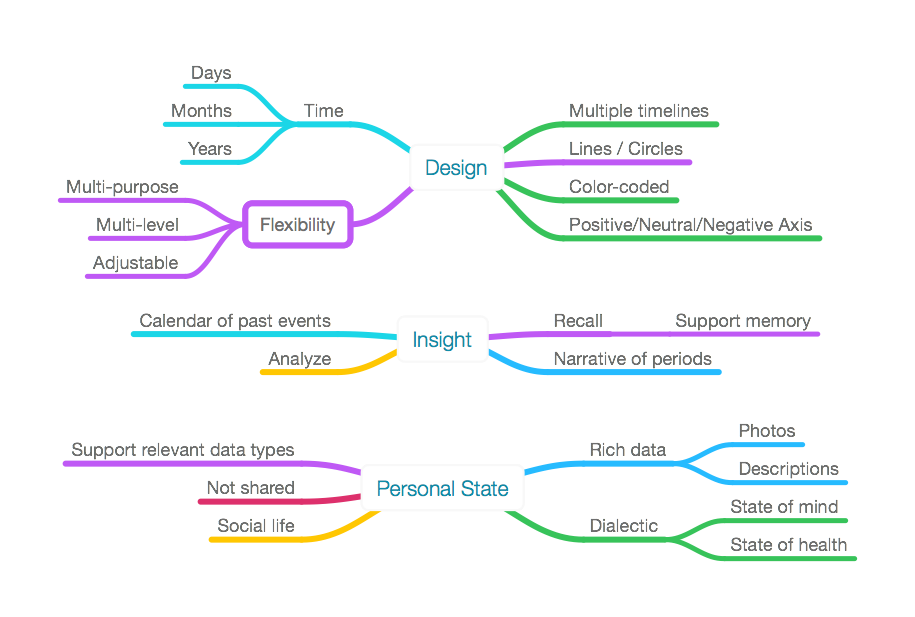
\includegraphics[width=1\linewidth]{Images/ThematicAnalysis}
    \caption{Workshop 1: Thematic Analysis}
    \label{fig:1}
\end{figure}

The themes describe issues and patterns that were prevalent in the dataset. However determining prevalence in such a short dataset was problematic. This lead to a reduced specificity in the themes. The thematic map has three main themes \textit{design, insight} and \textit{personal state}. Design contains information derived from the sketches and based on statements pertaining to their description of the sketches. Insight is related to the timelines and what the meaning, motivation and outcome such a timeline can provide. Personal state describes the participants main choice for visualization. The participants described their personal state on a holistic level, this qualitative measure was the measure against which other datatypes were considered.

These three main themes were selected because they could be separated by asking the question of how---design, why---insight and what---personal state. Braun and Clarke point to that themes should be ``internally coherent, consistent and distinctive''\cite[p.96]{Braun2006Using}. The three themes work well in their distinctiveness but less so in internal coherence and consistency. The qualitative codes worked here to describe subthemes, in subthemes which pointed to larger themes. But in doing so there were a range of qualitative choices about groupings which lead to further confusions.

The findings here are lacking in accuracy and absolutenss due to the number of participants combined with the short-interview time. This was made worse by using participatory sketching where the participant devoted several minutes drawing. Two of the groups were largely consistent and adopted each others ideas while one group were more independent. This was harder to consider when coding since the social dynamics within the participant groups remain unclear. 

\subsection{Design}
Design includes subthemes related to the visual and technical properties described by and sketched during the workshop. Several participants described how they would ``click-in'' in the timeline to expand the view from a year to a month, or from a month to a day. This ability to view and scale the timeline was related to working with different types of focuses. From short-term logging to long-term analysis. This was also expressed as a flexibility of the timeline. Such a tool should allow you to compare different types of data and have more than one purpose. For instance one participant wanted to log pain on a 1-10 scale while logging data about both activity levels and activity types. The point being to look at patterns of activities and activity levels that stress and produce a pain reaction.

Other participants described how documenting was related to their personal needs---``how my body works, if there is a lot of pain, if there is abrasions, if I sleep well, such things that are important for me to maintain control over''. These statements with others were interpreted as a need for a multi-purpose and adjustable timeline. Many of the participants also drew multiple views. Where they had a timeline with datapoints and then another view containing more specific information about that datapoint.

Lastly the participants used normal conventions such as smily/sad faces for good/bad and red/grey/green for negative, neutral and positive. There were little similarities between the sketches in terms of visual symbols. Several participants included more than one type of data in the timeline for comparison.  
\subsection{Insight}
Insight is the themes containing subthemes and data items related to the motivation, purpose and outcome for working with the proposed tool. Several participants mentioned using the timeline as a memory device for recall. Other talked about the analytical possibilities, here the participant describes a use-case without considering the technical and practical concerns: ``you could go in to special days where you see that something special happened\dots What did I do there, that day? Why did it fall? Learn from your mistakes\dots''. The same participant described another use where there is a part of the timeline covering a happy period. Here the participant thought of this as a reminder ``I want something I can look at. Like looking back at this here (points to high-point on sketch)\dots I was glad and my form was good and I know I cant there again that means alot''. 

One participant described the timeline as a ``calendar of past events''. Several participant mentioned recalling and answering questions related to their health. Here the timeline could be used to log and provide narratives of periods with difficulties or for instance with new medications. More simply one group wanted it to use when ``visiting the doctor and then they ask how have you been the last 6 months and you kind of don't know''. One participant mentioned a journal she had kept to log here stay at the hospital: ``there are many times I have gone and looked at the book at what happened then. A bit to reminisce (neutrally)''. In this context the timeline would be more of a narrative tool than a visualization and it should strive to accurately and truthfully represent the users life-worlds. 
\subsection{Personal state}
Personal state is used here to liberally contain themes related to the holistic sense of wellness. The participants described and sketched several different datatypes such as pain, activity and happiness. These datatypes were however always compared back to the overall state of being. Several participants included this as their main timeline. With an vertical axis of postive, neutral and negative personal states. There was an intentional ambiguity that one participant expressed as ``feelings and health (form) are two separate things\dots but of course they interact'' another expressed it as ``I could have written alot here but its in a way, mind and mood''. 

The participants largely described personal state as a dialetic over time where one day was clearly positive and another negative. The personal state could be summarized as the answers to the question: ``How are you?''. When probed the participants described how each datapoint could contain photos, notes, descriptions, colors to clarify and provide context. Several participants described this qualitative data as neccessary to understand extremes or sudden changes. They also proposed that social activities and friendships could be included as they were integral to their \textit{state of mind}. One group considered sharing the data in the app, but quickly realized that it was to personal. It's proposed purpose and strenght depend upon its ability to be personal. 

Participants described logging data types relevant to their specific needs. As previously mentioned two participants wanted to log pain, training, activity and abrasions while others mentioned medicines, sleep and mood. Largely they described the two types, simple numerical scales and qualitative data. 

\subsection{Discussion of the results}
In workshop 1 there were eight participants that each sketched a timeline. From reviewing the transcription it became clear that the sketching exercise was started without steering and ended rather quickly. This was done because of the time and the participants. Largely the sketches worked to engage and start the discussion. Of the 8 participants 1 sketched a drawing without any meaningful content, the other 7 participants all made original contributions of varying quality and fidelity. Most of the sketches are crude and simple but they describe and show several instering aspects. However due to the very short time period they were made in they should not be considered as prototypes but as objects-of-discussion. 
During the sketching session the participants contributed with several original ideas and where more open to qualitative data than expected. It is however unclear if they will find logging and using such data as meaningful.

From visualization literature and research there has been little concentration on mixing qualitative data with automated visualizations. (mer her)

Based on the result from the workshop it became clear to me that the focus should be towards expressing some aspect of the participants life-world that can provide insight. There should be less emphasis on the transforming the data to visualize meanings or patterns and instead focus on providing long-term and short term narratives. In the analysis it became clear that the participants wanted some focus on their \textit{personal state}. 
This points to two alternatives, a standard timeline of personal state combined with other data or a timeline customized for insight. 

The first alternative is a timeline that shows a simplified \textit{personal state} visualized over time, with other qualitative or quantitative data such as images, notes or other annotation illustrated but not shown on the main timeline. This timeline would have different views based on the time perspective--- day, month or year. It could also support several data types such as mood, pain or energy.

The second alternative is less clear but would entail a customization where each users can create different datatypes they want to log. The datatypes then describe for that users their self-defined progressive \textit{personal state}. For instance two participant mentioned logging pain as especially useful. For them this may be their primary focus, however it could/should be combined with other datatypes such as \textit{personal state} or activity level. 

Other alternatives that were included in the sketches were calendars, reminders, logging food. At this point such features are less interesting as they are not directly related to the research questions. 


\end{document}